\chapter{Testes e Resultados}\label{cap:conclusão}
Neste capítulo são detalhados os testes de desenvolvimento e performance do aplicativo jogo e uma descrição e resultados dos testes práticos com crianças.

\section{Testes de Desenvolvimento}


\subsection{\textbf{Testes de Tempo de Resposta do Reconhecimento}}



\subsection{\textbf{Teste de Taxa de Assertividade}}


\section{Testes Práticos}

\subsection{\textbf{Descrição}}


A metodologia de teste com crianças proposta pelos pesquisadores foi submetida e obteve a aprovação do comitê de ética. Portanto, antes de iniciar as etapas descritas abaixo, foi apresentado aos participantes os objetivos e a metodologia da pesquisa. A participação foi  realizada apenas após a assinatura do Termo de Consentimento Livre e Esclarecido (TCLE) pelos responsáveis. Os participante também receberam uma via do TCLE assinado pelo pesquisador responsável. Os dados pessoais coletados, como nome e idade, serão acessados apenas pela equipe de pesquisa. Todos os dados serão destruídos, no prazo de, no máximo, 1 ano.

Pensando nas eventualidades causadas pelo vírus Sars-CoV-2, causador da pandemia mundial do covid-19 no ano de 2020, os testes descritos abaixo foram realizados integralmente seguindo as orientações da OMS \cite{oms_2020} de prevenção ao Sars-CoV-2.

Os testes práticos foram realizados em duas etapas. A primeira etapa foi a resolução dos desafios propostos pelo jogo e a segunda etapa foi a resposta ao questionário de pesquisa criado pelos pesquisadores. A primeira etapa foi realizada pela criança e a segunda etapa pode ser realizada pela criança com, ou sem, o auxílio de um responsável que tenha acompanhado a aplicação da primeira etapa. Os testes foram realizados com X participantes.

Na primeira etapa os participantes jogaram o jogo dentro do ambiente de sua escolha. Os pesquisadores foram até o local de aplicação para disponibilizar os blocos físicos, celular com o aplicativo e explicar o
funcionamento do jogo para os responsáveis e as crianças. A aplicação da primeira foi será supervisionada pelos responsáveis e pesquisadores. Os participante jogaram o  aplicativo jogo por um tempo entre 15 a 30 minutos.

Na segunda etapa da pesquisa, o participante respondeu  a um questionário online que foi disponibilizado após o término da primeira etapa e ficou disponível por uma semana. O objetivo foi  validar a efetividade do aplicativo jogo em relação ao engajamento do participante, competência em ensinar programação e
capacidade de ensinar sobre reciclagem. Foi disponibilizado ao participante ou responsável, por meio do Whatsapp ou e-mail, o link do questionário. O questionário possui 5 perguntas obrigatórias e estima-se que o tempo de preenchimento do questionário seja de aproximadamente 15 minutos. As perguntas são: 1 - Qual seu primeiro nome ?; 2 - Qual a sua idade ? 3 - Você se sentiu motivado a continuar jogando o jogo ? Na pergunta 4 e 5, foram mostradas ao respondente, a imagem de um labirinto Figura \ref{figura:q4}, semelhante ao do jogo, e uma imagem de uma garrafa plástica Figura \ref{figura:q5} respectivamente, todas com 4 alternativas , das quais apenas uma é correta. 4 - Qual sequência corresponde a resolução do labirinto abaixo? a) $\uparrow,  \leftarrow, \uparrow, \rightarrow$ ; b) $\uparrow, \leftarrow, \leftarrow, \uparrow, \rightarrow, \rightarrow, \rightarrow, \rightarrow$; c) $\uparrow, \leftarrow, \leftarrow, \uparrow, \rightarrow, \rightarrow, \rightarrow$; d) $\leftarrow, \leftarrow, \uparrow, \rightarrow, \rightarrow, \rightarrow, \rightarrow$; 5 - Em qual das lixeiras você descartaria o lixo abaixo? a) Imagem de uma lixeira azul; b) Imagem de uma lixeira amarela; c) Imagem de uma lixeira vermelha; d) Imagem de uma lixeira verde.

\begin{figure}[H]
    \caption{Pergunta 4}
    \centering
    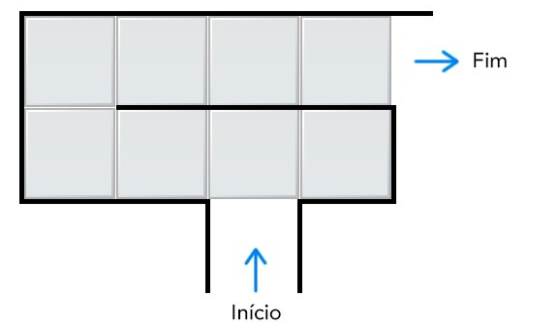
\includegraphics[width=10cm]{Imagens/Cap5/Q4.png}
    \legend{\small{Fonte: os autores (2020)}}
    \label{figura:q4}
\end{figure}


\begin{figure}[H]
    \caption{Pergunta 5}
    \centering
    
\includegraphics[width=10cm]{Imagens/Cap5/Q5.png}
    \legend{\small{Fonte: os autores (2020)}}
    \label{figura:q5}
\end{figure}

\subsection{\textbf{Teste com Crianças}}


\section{Conclusão}

Neste trabalho foi estudado a falta de recursos tecnológicos de baixo custo e fácil utilização para educação básica. Além disso, pensando nas profissões do futuro, foi visto a importância do ensino de lógica de programação para as crianças de hoje (2020).
Pensando nesses problemas apresentados, foi proposto e desenvolvido um aplicativo que tem o objetivo de tentar ensinar programação para crianças do ensino básico e fundamental 1. O aplicativo é um jogo que interage com blocos físicos por meio de reconhecimento de imagem. O aplicativo consiste em um jogo com o tema de reciclagem no qual por meio de blocos físicos, com instruções de andar, virar, esperar, repetir e blocos numerados de 0 a 9, a criança deve resolver desafios de lógica proposto pelo jogo organizando esses blocos em sequências lógicas, fotografando e submento pelo aplicativo para validar se suas instruções estão corretas ou não. O aplicativo foi desenvolvido em Unity e Python3 e os blocos foram impressos por uma impressora 3D e coloridos manualmente com tinta. O resultado final do aplicativo atendeu à todos os requisitos que foram propostos no Capítulo \ref{cap:intro} deste trabalho.

Após o término do desenvolvimento do aplicativo jogo, foram realizados teste com crianças. O objetivo destes testes foram analisar a capacidade do aplicativo jogo em reter a atenção da crianças, capacidade de ensinar conceitos básicos de programação e competência de ensinar sobre reciclagem.

Durante o desenvolvimento do aplicativo jogo, foi identificado identificado algumas possibilidades de otimização para este trabalho, como por exemplo a escolha das cores dos blocos. Por meio dos testes práticos, foi observado que a cor amarelo não se comporta bem na etapa de reconhecimento de imagem pois quando é exposta diretamente a luz tem seus parâmetros de RGB facilmente distorcidos.

\clearpage

\section{Trabalhos Futuros}

Após a conclusão do trabalho, foi identificado também possibilidade de continuações para trabalhos futuros. Como possíveis trabalhos futuros, pode-se apontar:

\begin{enumerate}
    \item Desenvolvimento do aplicativo para outros sistemas operacionais, como o iOS. 
    
    \item Desenvolvimento de novos tipos de blocos.
    
    \item Desenvolvimento de novas fases que utilizem mais blocos ou até mesmo outros tipos de blocos.
    
    \item  Refinar o algoritmo de reconhecimento dos blocos para reconhecer blocos desenvolvidos com outros materiais, desta forma, seria possível disponibilizar um pdf com instruções de montagem de blocos e desta forma a própria criança, por meio desse passo a passo, poderia construir seus blocos com papel, deixando assim a solução ainda mais econômica.

    
\end{enumerate}









